\documentclass[UTF8,10pt,aspectratio=169]{ctexbeamer}

\usepackage{amsmath, amssymb}
\usepackage{tikz}
\usetikzlibrary{calc}
\usepackage{newtxtext, newtxmath} % 经典试卷西文与公式字体

% ==================== 极简试卷感风格 ====================
\usetheme{default}
\usecolortheme{default}
\usefonttheme{serif} % 强制使用衬线体，形成“试卷感”
\setbeamertemplate{navigation symbols}{}
\setbeamertemplate{footline}[frame number]

% ==================== 常用格式命令 ====================
\newcommand{\courseTitle}{这里填写课题}
\newcommand{\courseSubtitle}{这里填写课型或学案编号}

\newcommand{\answer}[1]{%
	\textbf{【答案】} #1%
}

\newcommand{\analysis}[1]{%
	\vspace{0.2cm}
	\textbf{【详解】} #1%
}

\newcommand{\proofblock}[1]{%
	\vspace{0.2cm}
	\textbf{【证明】} #1%
}

\newcommand{\methodnote}[1]{%
	\vspace{0.2cm}
	\textbf{【方法小结】} #1%
}

\title{\courseTitle}
\author{}
\date{}

\begin{document}

% ==================== 封面 ====================
\begin{frame}
	\titlepage
	\begin{center}
		{\Large \textbf{\courseTitle}}

		\vspace{0.5cm}
		{\large \courseSubtitle}
	\end{center}
\end{frame}

% ==================== 题目页：基础样式 ====================
\begin{frame}
	1. 这里填写题目正文。可以直接写选择题、填空题或解答题。

	\vspace{0.3cm}
	A. 选项一 \quad B. 选项二 \quad C. 选项三 \quad D. 选项四

	\pause
	\vspace{0.3cm}
	\answer{这里填写答案}

	\analysis{
		这里填写解析。解析可以分行书写，也可以使用行间公式：
		\[
			这里填写关键公式。
		\]
	}
\end{frame}

% ==================== 题目页：带 TikZ 图形 ====================
\begin{frame}
	2. 这里填写带图形的题目正文。

	\vspace{0.2cm}
	\begin{center}
		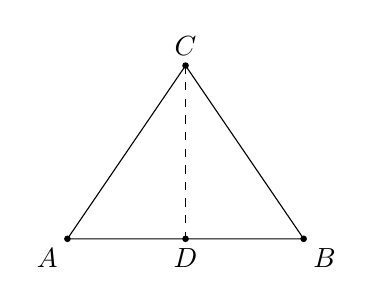
\begin{tikzpicture}[scale=1.0]
			\coordinate (A) at (0,0);
			\coordinate (B) at (3,0);
			\coordinate (C) at (1.5,2.2);
			\coordinate (D) at ($(A)!0.5!(B)$);

			\draw (A)--(B)--(C)--cycle;
			\draw[dashed] (C)--(D);
			\fill (A) circle (1.2pt);
			\fill (B) circle (1.2pt);
			\fill (C) circle (1.2pt);
			\fill (D) circle (1.2pt);

			\node[below left] at (A) {$A$};
			\node[below right] at (B) {$B$};
			\node[above] at (C) {$C$};
			\node[below] at (D) {$D$};
		\end{tikzpicture}
	\end{center}

	\pause
	\answer{这里填写答案}

	\analysis{
		这里填写解析。建议突出“为什么想到这个方法”，而不只是写运算。
	}
\end{frame}

% ==================== 证明题样式 ====================
\begin{frame}
	3. 这里填写证明题题目。

	\[
		这里填写需要证明的结论。
	\]

	\pause
	\proofblock{
		这里填写证明过程。
	}
\end{frame}

% ==================== 方法小结页 ====================
\begin{frame}
	\begin{center}
		{\Large \textbf{方法小结}}
	\end{center}

	\vspace{0.3cm}
	\begin{enumerate}
		\item \textbf{结构识别}：这里填写本节课最核心的题目结构。
		\item \textbf{常用工具}：这里填写主要方法。
		\item \textbf{易错边界}：这里填写学生容易误用的地方。
	\end{enumerate}
\end{frame}

\end{document}

